\chapter{交換對稱性、自旋與兩個負號}

\section{殼層填充與自旋--統計問題}

殼層模型的回顧從電子的兩項性質談起。電子的自旋為二分之一，兩個無量綱自旋投影為
\begin{equation}
m_s=+\frac12,
\qquad
m_s=-\frac12,
\end{equation}
而且電子遵守泡利不相容原理。這兩項事實彼此相關，但並非同一個陳述。

``同一狀態''這個說法需要謹慎理解。兩個電子不能佔據同一個完整的單粒子態。不過，若自旋態不同，兩個電子仍可共享同一個空間軌域。在氦原子的獨立電子近似中，兩個電子都佔據最低的空間軌域，一個自旋向上，另一個自旋向下。更精確地說，``第一個自旋向上、第二個自旋向下''與``第一個自旋向下、第二個自旋向上''這兩種可能性，屬於同一個糾纏的雙電子自旋態。

這只是舊殼層模型中的近似。它忽略電子間的交互作用，在此僅用來說明簡單的計數。對鋰而言，前兩個電子以相反自旋填入最低的空間軌域。第三個電子不能進入前述任一完整態，必須佔據較高能的軌域。

接下來看熟悉的軌道角動量圖。具有
\begin{equation}
\ell=0,\qquad \ell=1,\qquad \ell=2
\end{equation}
的扇區分別稱為\(S\)、\(P\)與\(D\)態。固定的\(\ell\)值對應
\begin{equation}
2\ell+1
\end{equation}
個軌道態，因此
\begin{equation}
\ell=0\Rightarrow 1,
\qquad
\ell=1\Rightarrow 3,
\qquad
\ell=2\Rightarrow 5.
\end{equation}
庫侖問題還有額外的簡併：不同\(\ell\)扇區的徑向能階可能具有相同能量。就殼層填充的論證而言，下一個殼層包含一個\(S\)軌域和三個\(P\)軌域，因此共有
\begin{equation}
1+3=4
\end{equation}
個空間態。自旋使態數加倍：
\begin{equation}
2(1+3)=8.
\end{equation}

從鋰到氖，這八個完整的單電子態依序填滿。閉殼層之後，鈉又有一個外層電子，因此在這個粗略圖像中，鈉與鋰相似。這裡要說的不是化學；重點是半整數自旋與不相容原理同時出現。

光子提供了對照。光子的自旋為整數，也不遵守不相容規則。經典電磁波對應於許多光子佔據同一個模式。玻色子可以聚集在同一個態中，而全同費米子不能重複佔據同一個完整態。問題是，這兩種配對有沒有可能相反：半整數自旋卻沒有不相容性，或整數自旋卻有不相容性？在三維空間中，自旋--統計關係給出的答案是否定的。這個熟悉的說法在一維與二維空間中需要加上限定；此處不嘗試證明場論中的結果。

\begin{classroomqa}
\lecturetimestamp{00:11:48}
\audiencequestion{玻色子能佔據同一個態的量子數有上限嗎？}
\lecturerresponse{沒有。玻色子的佔據數沒有上限，而且它們傾向於聚集在同一個態中。}
\end{classroomqa}

\section{多粒子波函數}

接下來透過兩個負號來理解兩者的關聯：一個來自交換，另一個來自旋轉。先從交換談起，暫時不考慮自旋。

令\(x_i\)表示粒子\(i\)的位置。下標表示粒子標記，不是笛卡兒分量；三個空間座標合併寫成符號\(x_i\)。\(n\)個粒子的位置基底為
\begin{equation}
\lvert x_1,x_2,\ldots,x_n\rangle.
\end{equation}
對於抽象態\(\lvert\Psi\rangle\)，座標波函數為
\begin{equation}
\psi(x_1,x_2,\ldots,x_n)
=
\langle x_1,x_2,\ldots,x_n\mid\Psi\rangle.
\end{equation}
其絕對值平方
\begin{equation}
\bigl\lvert\psi(x_1,x_2,\ldots,x_n)\bigr\rvert^2,
\end{equation}
是聯合機率密度，表示在\(x_1\)找到粒子\(1\)、在\(x_2\)找到粒子\(2\)，依此類推。

現在假設這些粒子是全同粒子。先想像把一個電子塗成藍色，另一個塗成紅色。如此一來，``藍色電子在\(x_1\)、紅色電子在\(x_2\)''，就能和``藍色電子在\(x_2\)、紅色電子在\(x_1\)區分開來。''實際的電子沒有這些顏色，也沒有個別標籤。交換用來記帳的標籤，並不會產生新的物理排列。

整體相位不會改變機率或期望值。因此，若態具有確定的交換行為，其座標波函數可以滿足
\begin{equation}
\psi(x_2,x_1)=\eta\,\psi(x_1,x_2),
\qquad
\lvert\eta\rvert=1.
\end{equation}
對同一次交換作用兩次，會恢復原來的自變數，並得到
\begin{equation}
\eta^2=1,
\end{equation}
因此，可能的兩個交換本徵值為
\begin{equation}
\eta=+1
\qquad\hbox{or}\qquad
\eta=-1.
\end{equation}

\editorialnote{只有在先假設態具有確定的交換行為之後，雙重交換的代數關係才能決定可能的本徵值。至於同一種類粒子的允許態必須屬於同一個交換扇區，這是額外的物理規則，不能單靠\(\eta^2=1\)推出。下文的不相容原理論證也有相同的限定：選定費米子扇區後，反對稱性會導出不相容性；但交換代數本身並不會選出該扇區。}

玻色子的允許波函數是對稱的，
\begin{equation}
\psi_B(x_1,x_2)=\psi_B(x_2,x_1),
\end{equation}
費米子的允許波函數則是反對稱的，
\begin{equation}
\psi_F(x_1,x_2)=-\psi_F(x_2,x_1).
\end{equation}
負號若乘上整個態，便無法直接觀察；但在振幅相加時，這個負號就會產生影響。交換對稱性正是藉此帶來可觀測的後果。

\section{乘積、加總與不相容原理}

先考慮兩個粒子都處於同一個單粒子軌域\(\psi_0\)。它們的乘積為
\begin{equation}
\psi_0(x_1)\psi_0(x_2).
\end{equation}
交換粒子座標後得到
\begin{equation}
\psi_0(x_2)\psi_0(x_1)
=
\psi_0(x_1)\psi_0(x_2).
\end{equation}
波函數的值是數，不是算符，因此各因子可以交換次序。同一態的乘積是對稱的，這是玻色子允許的形式，但不能描述兩個全同費米子。

接著讓兩個粒子分別處於不同的單粒子軌域：
\begin{equation}
\psi_0(x_1)\psi_1(x_2).
\end{equation}
交換後得到
\begin{equation}
\psi_0(x_2)\psi_1(x_1).
\end{equation}
若兩個函數不同，交換後的乘積通常既不等於原式，也不等於原式的負值。因此，單獨的乘積不具備所要求的交換對稱性。這並不表示一個粒子不能佔據\(\psi_0\)而另一個粒子佔據\(\psi_1\)；而是說，雙粒子態必須把這兩種粒子分配方式組合起來。

對稱組合為
\begin{equation}
\psi_B^{(01)}(x_1,x_2)
\propto
\psi_0(x_1)\psi_1(x_2)
+
\psi_0(x_2)\psi_1(x_1),
\end{equation}
反對稱組合為
\begin{equation}
\psi_F^{(01)}(x_1,x_2)
\propto
\psi_0(x_1)\psi_1(x_2)
-
\psi_0(x_2)\psi_1(x_1).
\end{equation}
交換論證不需要歸一化，因此比例符號已足夠。兩個態都各有一個粒子處於每個軌域；差別只在於如何組合這兩種不可區分的分配方式。

現在令兩個軌域重合。玻色子的組合變成
\begin{align}
\psi_B^{(00)}(x_1,x_2)
&\propto
\psi_0(x_1)\psi_0(x_2)
+
\psi_0(x_2)\psi_0(x_1)\\
&=
2\psi_0(x_1)\psi_0(x_2),
\end{align}
這個結果不為零。費米子的組合則是
\begin{align}
\psi_F^{(00)}(x_1,x_2)
&\propto
\psi_0(x_1)\psi_0(x_2)
-
\psi_0(x_2)\psi_0(x_1)\\
&=0.
\end{align}
由反對稱交換規則便可得到不相容性：不存在兩個費米子處於同一個單粒子態的非零反對稱態。

對多粒子態而言，這項規則適用於任意兩個自變數的對換。對換後，玻色子的波函數保持不變，費米子的波函數則改變符號。再做一次相同的對換，兩者都會回到原狀。令人意外的是，單次交換雖不改變任何可觀測的粒子標籤，卻會改變費米子態的符號。

\section{完整粒子標記中的自旋}

現在只要稍作調整，就能把自旋納入。單粒子振幅同時依賴位置與離散的自旋標記，
\begin{equation}
\psi(x,\sigma),
\end{equation}
其中\(\sigma=+1\)或\(-1\)表示所選\(\sigma_z\)測量結果的標記。其絕對值平方是指定位置與自旋標記的聯合機率密度。

對多粒子而言，波函數為
\begin{equation}
\psi(x_1,\sigma_1;\,x_2,\sigma_2;\,\ldots).
\end{equation}
交換時，兩個粒子所屬的一切都要互換，不只有位置：
\begin{align}
\psi_B(x_1,\sigma_1;\,x_2,\sigma_2)
&=
+\psi_B(x_2,\sigma_2;\,x_1,\sigma_1),\\
\psi_F(x_1,\sigma_1;\,x_2,\sigma_2)
&=
-\psi_F(x_2,\sigma_2;\,x_1,\sigma_1).
\end{align}
這就是開頭殼層模型所述內容的精確形式。只有在完整態（包括自旋）不同時，兩個電子才能共享同一個空間軌域。

\begin{classroomqa}
\lecturetimestamp{00:34:33}
\audiencequestion{交換對稱性是置換群的一種情形嗎？}
\lecturerresponse{是。交換粒子是一種置換，而正號或負號的變換律構成置換群的一個表示。}
\end{classroomqa}

\begin{classroomqa}
\lecturetimestamp{00:35:12}
\audiencequestion{為什麼雙粒子態是單粒子波函數的乘積，而不是和？}
\lecturerresponse{和描述的是一個粒子的疊加態。乘積屬於雙粒子張量積空間，描述兩個粒子分別處於各自的單粒子態。}
\end{classroomqa}

下方黑板展示了完整粒子標記的交換方式。\footnote{位置--自旋標記的排列，是根據可辨識的黑板畫面，以及00：33：43至00：34：25之間的講解重建而成。}
\begin{figure}[htbp]
\centering
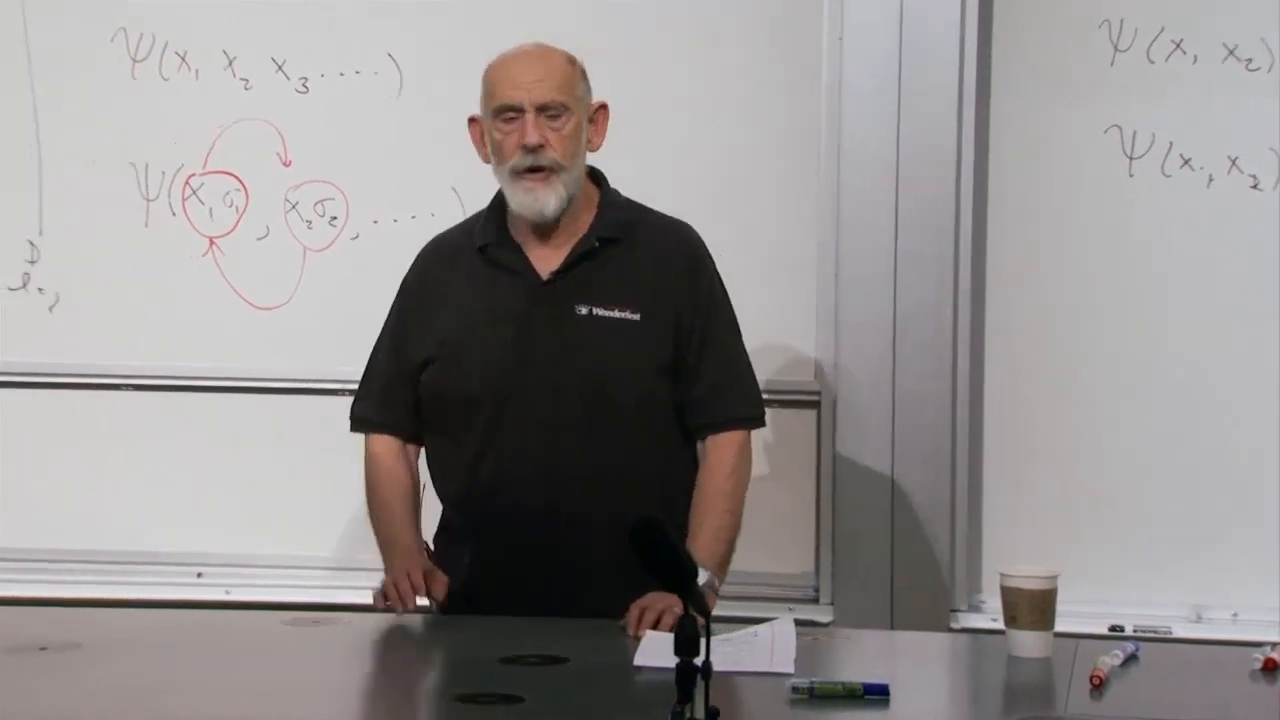
\includegraphics[width=0.9\linewidth]{lecture_05_frame_03.png}
\caption{交換兩個全同粒子時，兩者完整的位置--自旋標記也會互換。玻色子態保持不變，費米子態則改變符號。}
\lectureframe{00:35:25}
\end{figure}

這是線性疊加的兩種不同用法。對單一粒子而言，
\begin{equation}
\alpha\psi_0(x)+\beta\psi_1(x)
\end{equation}
表示兩種可能性的疊加。對兩個粒子而言，
\begin{equation}
\psi_0(x_1)\psi_1(x_2)
\end{equation}
則是在具有兩個粒子座標的空間中的乘積振幅。對稱化或反對稱化會將此乘積與交換後的對應項組合起來。

\begin{classroomqa}
\lecturetimestamp{00:36:13}
\audiencequestion{交換粒子會產生干涉效應嗎？}
\lecturerresponse{會。同一態的費米子振幅為零，可以理解為兩個交換項之間發生了相消干涉。}
\end{classroomqa}

\begin{classroomqa}
\lecturetimestamp{00:37:13}
\audiencequestion{泡利是用同樣的對稱性論證推導出不相容原理的嗎？}
\lecturerresponse{泡利從一項經驗事實出發，找到一個能表述該事實的數學架構。他起初並不是從更基本的理論推導出不相容原理。}
\end{classroomqa}

反對稱性提供了表述經驗性不相容規則的數學架構。

\begin{classroomqa}
\lecturetimestamp{00:39:01}
\audiencequestion{粒子交換干涉和不同可能路徑之間的干涉有關嗎？}
\lecturerresponse{有。一種可能的歷程是兩個粒子不交叉地通過，另一種則是兩者交叉，抵達交換後的位置。玻色子的振幅會相加，費米子的振幅則可能相消。}
\end{classroomqa}

交換帶來第一個負號，旋轉帶來第二個。

\section{第二個負號：旋轉 \texorpdfstring{\(2\pi\)}{2 pi}}

整周旋轉看起來似乎什麼也沒做。轉過角度\(2\pi\)後，每個一般的幾何方向都回到起點。然而，真正必須回到原狀的是機率與期望值。態向量本身可以帶著整體相位回到原狀，正如交換作用也可能使它帶上整體相位。

\begin{classroomqa}
\lecturetimestamp{00:42:12}
\audiencequestion{旋轉是繞哪一條軸進行？生成元是軌道角動量、自旋，還是兩者都有？}
\lecturerresponse{可以選擇一條外部軸；以下選用\(z\)軸。生成元是總角動量，包含軌道角動量與自旋的貢獻。自旋本身不必指向所選的軸。}
\end{classroomqa}

\editorialnote{本段討論的角動量公式採用\(\hbar=1\)，因此\(m\)是\(J_z\)的無量綱本徵值。}

令\(\psi(\theta)\)表示旋轉參數增加至角度\(\theta\)時所得到的態。依照此處採用的慣例，
\begin{equation}
J_z\psi(\theta)
=
-i\frac{\partial}{\partial\theta}\psi(\theta).
\end{equation}
對於具有確定\(J_z\)的態，
\begin{equation}
J_z\psi(\theta)=m\psi(\theta).
\end{equation}
合併這些方程式可得
\begin{equation}
-i\frac{\partial}{\partial\theta}\psi(\theta)
=
m\psi(\theta),
\end{equation}
解為
\begin{equation}
\psi(\theta)=e^{im\theta}\psi(0).
\end{equation}

\(m\)的允許值為整數或半整數。因此
\begin{equation}
\psi(2\pi)
=
\begin{cases}
+\psi(0), & m\in\mathbb Z,\\[4pt]
-\psi(0), & m\in\mathbb Z+\tfrac12.
\end{cases}
\end{equation}
再轉一整圈後，
\begin{equation}
\psi(4\pi)=\psi(0)
\end{equation}
兩種情況都成立。這就是第二個負號：半整數角動量多重態中的態，經過\(2\pi\)旋轉後會改變符號。

這個符號不會改變\(\lvert\psi\rvert^2\)，所以乘在整個態上時無法直接觀察。即便如此，對半整數自旋態而言，\(2\pi\)旋轉所代表的變換並非恆等變換。若能讓這個符號相對於另一個相干振幅產生差異，兩者的不同便可觀測。

\section{\texorpdfstring{\(2\pi\)與\(4\pi\)}{2 pi和4 pi}路徑}

無須進一步推導，就能看出\(2\pi\)與\(4\pi\)之間的差異。一手握住杯子，不放手地轉一整圈。杯子回到原來的朝向，但手臂扭轉了。再繼續轉一圈，手臂便能回到原來的位置，而不必反轉杯子的轉動。

另一種相關的演示，是把球放在盒子裡，再用繩子將球連到盒子。將球轉過\(2\pi\)後，繩子會纏結。在一般的三維空間中，\(4\pi\)轉動所形成的纏結可以解開。關鍵不只是球最後的朝向，而是球在旋轉空間中走過的路徑。

\begin{classroomqa}
\lecturetimestamp{00:54:22}
\audiencequestion{如果球繞同一軸轉兩圈，繩子真的能解開嗎？這需要另一個空間維度嗎？}
\lecturerresponse{\(4\pi\)路徑可以在一般三維空間中解開。時間用來描述運動，不是另一個空間方向。\(2\pi\)路徑無法以這種方式解開，而\(4\pi\)路徑則可以。}
\end{classroomqa}

這些演示呈現了非平凡的\(2\pi\)路徑與可解開的\(4\pi\)路徑之間的差異，無須進一步建立旋轉群的形式理論。

\section{皮帶圖像中的交換與旋轉}

現在可以並列看這兩個負號。交換兩個全同費米子會使其聯合波函數改變符號。將半整數自旋態旋轉\(2\pi\)，也會使其改變符號。皮帶圖像呈現了這兩種操作之間的幾何關聯。

安排皮帶，使下方兩端互相交換。從另一個角度看，同一條皮帶帶有\(2\pi\)的扭轉。若同時進行交換與\(2\pi\)旋轉，扭轉便會消失，留下未扭轉的皮帶。這個組合過程可以連續變形為什麼也不做。\footnote{講座中將交換--旋轉的觀察歸功於David Finkelstein。來源紀錄未指出具體出版物，因此此處只保留講座中的這項歸屬。}

\begin{classroomqa}
\lecturetimestamp{01:01:12}
\audiencequestion{這只是描述皮帶如何嵌入空間，還是也在描述粒子的拓撲？}
\lecturerresponse{皮帶也可以解讀為時空中的粒子歷程。若時間軸朝上，取皮帶的橫截面便會得到類粒子物體。成對的物體被產生，其中一個旋轉\(2\pi\)，接著兩個全同物體互相交換。在這段歷程中，旋轉相位與交換相位彼此抵消。}
\end{classroomqa}

這段歷程清楚呈現了相位的計算方式。起初沒有粒子。在兩個分開的位置各產生一個粒子--反粒子對，因此在中間時刻共有四個粒子。讓其中一個粒子旋轉\(2\pi\)，同時在系統的另一處交換兩個全同粒子。整段歷程可以變形為最基本的歷程：產生一對粒子，之後再將其湮滅。依照此處討論的符號計算，這段平凡歷程不會多出相位。若以\(\eta_{\mathrm{rot}}\)和\(\eta_{\mathrm{ex}}\)表示這兩個符號，講述中的抵消關係可簡潔寫成\footnote{此相位方程式記錄了01：06：50至01：07：18所描述的抵消；講座將這個構造作為啟發性的說明，而非嚴格證明。}
\begin{equation}
\eta_{\mathrm{rot}}\eta_{\mathrm{ex}}=1.
\end{equation}

\begin{classroomqa}
\lecturetimestamp{01:03:34}
\audiencequestion{能不能讓兩個粒子各自移動\(\pi\)，再重新調整它們的方向，藉此將交換和旋轉連結起來？}
\lecturerresponse{這種構造或許反映了相關的數學，但其中使用了兩次各自獨立的\(\pi\)旋轉。此處分析的過程只包含一次\(2\pi\)旋轉，因此兩種論證並不相同。}
\end{classroomqa}

這個論證以粒子類物體能夠被產生和湮滅為前提。若理論中的粒子永恆存在，論證就不會採用這種形式。這也不是自旋--統計定理的標準證明。它的目的，是呈現交換與旋轉的符號彼此吻合的一個拓撲理由。

\section{團塊、鏡像與湮滅}

這個構造也可以用局域場組態來呈現。假設一個或多個場幾乎處處都取真空值，但在某個小區域內具有非零的形狀與結構。這種局域組態稱為團塊。

接著構造第二個組態，使它成為第一個組態適當的鏡像。稱其中一個為粒子，另一個為反粒子。讓兩者靠近，使場組態中彼此對應的部分相遇並相互抵消。在過程中，團塊的某些部分可能已經消失，其他部分仍然存在。繼續變形，剩餘結構也會消失，場便回到真空組態。皮帶上兩個方向相反的扭轉也呈現相同的圖像：將扭轉推到一起，它們便會解開。

這個過程也可以反向進行。空間可以產生一個團塊及其鏡像夥伴。可以產生兩對這樣的物體，將其中一個團塊旋轉\(2\pi\)，交換兩個全同團塊，然後再讓這些物體對湮滅。同樣的交換--旋轉抵消關係也適用於此。這仍是對原構造的啟發式延伸，並非適用於每種局域激發的定理。

\begin{classroomqa}
\lecturetimestamp{01:11:30}
\audiencequestion{有沒有這類團塊場組態的實際例子？}
\lecturerresponse{有。例如，Skyrmion模型描述中的原子核、磁單極子，以及場的其他類粒子激發。}
\end{classroomqa}

鏡像團塊的圖像有助於理解這種推廣。關鍵不在於物體起初是不是基本點粒子，而在於一個類粒子激發及其夥伴能否連續地被產生、彼此靠近並湮滅。這項特性引出旋轉行為與交換行為之間更廣泛的關係。

\begin{classroomqa}
\lecturetimestamp{01:16:12}
\audiencequestion{自旋為二分之一，是否表示態累積的旋轉相位只有通常的一半？}
\lecturerresponse{依照此處的慣例，相位為\(e^{im\theta}\)。對半整數的\(m\)而言，旋轉\(2\pi\)會得到\(-1\)，旋轉\(4\pi\)則會得到\(+1\)。}
\end{classroomqa}

\section{整體符號與零結果實驗}

\(2\pi\)旋轉產生的負號能觀測到嗎？先看一個無法觀測到它的實驗。將電子囚禁在磁場中，緩慢轉動裝置\(2\pi\)，讓電子自旋跟隨磁場，接著將電子釋放到干涉裝置中。再與未進行旋轉、其餘步驟相同的實驗比較。

旋轉使態變為
\begin{equation}
\psi\longmapsto-\psi,
\end{equation}
但負號乘在整個態上，因此所有機率都不變。最終的干涉圖樣不會留下是否曾進行預備旋轉的任何痕跡。這是零結果實驗：共同相位沒有另一個振幅可供干涉。

\begin{classroomqa}
\lecturetimestamp{01:20:01}
\audiencequestion{為什麼磁場必須緩慢旋轉？}
\lecturerresponse{自旋必須持續跟隨旋轉中的磁場。如果磁場轉得太快，自旋就無法持續與磁場保持同步。}
\end{classroomqa}

\section{單一電子的兩個相干分支}

若能讓符號成為相對相位，便可以觀測到它。讓一個電子通過分束器，使它的波函數一部分沿一條路徑前進，另一部分沿另一條路徑前進：
\begin{equation}
\psi(x)=\psi_1(x)+\psi_2(x).
\end{equation}
這是一個電子，不是兩個電子。它處於兩種可能性的相干疊加態。必須清楚區分：這兩個波包不是兩個獨立的粒子。

將兩個波包分別引導到有磁場的區域。在其中一個區域內將磁場旋轉\(2\pi\)，另一個區域則保持不變。對半整數自旋態而言，
\begin{equation}
\psi_1(x)+\psi_2(x)
\longmapsto
\psi_1(x)-\psi_2(x),
\end{equation}
此處將被旋轉分支的標記選為\(2\)。現在符號成為相對的。兩個波包隨後重疊時，原本相加的振幅便改為相減。原本發生相長干涉的位置可能變成相消干涉的位置，甚至形成節點。

\begin{classroomqa}
\lecturetimestamp{01:23:46}
\audiencequestion{只有一個電子，卻有兩個波函數分支；究竟是哪個部分在旋轉？}
\lecturerresponse{電子處於兩個局域化可能性的相干疊加態。一個分支經過旋轉，另一個則沒有。若打開盒子確認電子位於哪個分支，這項測量就會破壞干涉。}
\end{classroomqa}

打開盒子只會看見一個電子，位於其中一個盒子裡。若不進行這項測量，兩個振幅都會保留在態中。重複實驗，探測結果便會逐次累積成干涉圖樣。在相對負號造成的節點位置，不會探測到電子。

\section{磁進動與雙縫干涉}

更實際的示意安排，可以取代極慢的盒子實驗。將相干電子波分成兩條路徑。在其中一條路徑上，讓電子通過磁場區域，且令其自旋初始方向與磁場垂直。接著自旋會進動。調整磁場強度與通過時間，就能讓該分支中的自旋完成一整個\(2\pi\)轉，而另一分支則不經歷這種轉動。\footnote{講座提到一項相關的旋量相位實驗已經進行，並說明其原理；但來源紀錄沒有指出論文或特定裝置。因此，此處僅依講座所述介紹這個構造。}

\begin{classroomqa}
\lecturetimestamp{01:27:05}
\audiencequestion{如何判定單一電子走過哪條路徑？}
\lecturerresponse{無法在不破壞實驗的情況下判定。任何記錄電子所走路徑的測量都會破壞干涉。}
\end{classroomqa}

\begin{classroomqa}
\lecturetimestamp{01:27:50}
\audiencequestion{波函數的分支究竟是什麼？分束器又如何產生兩個分支？}
\lecturerresponse{分支是沿某條路徑局域化的波包。分束器會將入射波分成兩個空間上分離的波包，電場或磁場則可以引導它們沿不同路徑前進。}
\end{classroomqa}

除了磁場區域之外，這就是雙縫實驗。入射電子波分成兩個波包。出射波擴展至共同的探測區域，振幅在此重疊。若沒有相對旋轉，中心處的振幅可能相加。在一條路徑中加入\(2\pi\)自旋旋轉，會使其中一個振幅反號，因而可能讓相同的貢獻互相抵消。

\begin{classroomqa}
\lecturetimestamp{01:30:46}
\audiencequestion{電子穿過不同的管子或狹縫，為什麼還會發生干涉？}
\lecturerresponse{最終的探測不會揭示電子走過哪條路徑。兩個出射波的振幅會在探測器處擴展並重疊。若查看電子走過哪條路徑，干涉就會被破壞。}
\end{classroomqa}

\begin{classroomqa}
\lecturetimestamp{01:33:22}
\audiencequestion{管子或狹縫的直徑必須與電子波長相當嗎？}
\lecturerresponse{若採用字面意義上以繞射為基礎的雙縫設計，開口必須夠小，才能產生所需的擴散。此處描述的是示意裝置，不是實際的設計方案。}
\end{classroomqa}

\begin{classroomqa}
\lecturetimestamp{01:33:44}
\audiencequestion{光子的偏振若也旋轉\(2\pi\)，干涉圖樣會保持不變嗎？}
\lecturerresponse{會。光子具有整數自旋，因此旋轉完整的\(2\pi\)不會引入費米子的負號。}
\end{classroomqa}

\begin{classroomqa}
\lecturetimestamp{01:34:12}
\audiencequestion{實際實驗與理想化版本之間有何細微差異？}
\lecturerresponse{理想的設計讓自旋絕熱地旋轉。在實際情況中，電子會穿過一個磁場區域，自旋進動得較快；不過，測得的相位仍是與旋轉\(2\pi\)一圈相應的相位。}
\end{classroomqa}

緩慢旋轉的設計確保自旋跟隨磁場，不會產生額外運動，藉此凸顯核心概念。進動的設計則透過動力學過程得到相同的相對符號。無論採用哪種設計，兩條路徑都必須變得不可區分，才能形成干涉圖樣。

\begin{classroomqa}
\lecturetimestamp{01:36:15}
\audiencequestion{分束之後，兩個分支必須重新合併嗎？}
\lecturerresponse{是。出射的波包必須彼此重疊，或擴展至共同的探測區域，振幅才能形成干涉圖樣。}
\end{classroomqa}

\begin{classroomqa}
\lecturetimestamp{01:38:12}
\audiencequestion{這個單電子旋轉實驗是泡利不相容原理的結果嗎？}
\lecturerresponse{不是。實驗中只有一個電子。測量的是旋轉時旋量的相位，而不是兩個費米子不能佔據同一個態。}
\end{classroomqa}

\section{交換干涉與相對旋轉}

原則上，同樣的一般方法也能顯示交換符號，不過所提議的裝置更為複雜。先取兩個電子，將它們的聯合波函數分成兩個相干分支。電子仍然只有兩個，不是四個：這一對電子會沿著兩種可能路徑之一演化。在一個分支中交換兩個電子，在另一個分支中則不交換。兩個分支重新合併後，費米子的交換符號會表現為相對相位，並可能改變干涉。

最後的設想直接比較這兩個負號。一個分支取得費米子的交換相位，另一個分支則取得相應的\(2\pi\)旋轉相位。兩者都是\(-1\)，因此相對效應會抵消。\footnote{從01:40:26到01:41:15的錄音清楚呈現了交換相位、\(2\pi\)旋轉相位及兩者的抵消，但根據現有錄音，無法確定旋轉具體如何安排。}講座將此描述為一項思想實驗，並表示據講者所知，這項實驗尚未實際進行。

\begin{classroomqa}
\lecturetimestamp{01:41:34}
\audiencequestion{觀察到交換相位，會對兩個電子的不可區分性構成挑戰嗎？}
\lecturerresponse{不會。量子力學中的不可區分性，比經典意義上的相同性更微妙。即使沒有任何可觀測的標籤能區分粒子，態向量在交換下仍可以改變符號。}
\end{classroomqa}

最後還有一項限定。若將整個孤立世界旋轉\(2\pi\)，只會產生一個共同相位，任何內部實驗都無法測出它。因此，可探測的實驗必須讓一個相干分支相對於另一個分支旋轉。觀察到的不是絕對符號，而是相對符號所造成的干涉。
